\documentclass[border=0pt]{standalone}
\usepackage{lmodern}
\usepackage{tikz}
\usepackage{pgfplots}
\usepgfplotslibrary{groupplots}
\pgfplotsset{compat=1.17}
\definecolor{f07min}{HTML}{000000}
\definecolor{f07sg}{HTML}{0072B2}
\definecolor{f07arpls}{HTML}{D55E00}
\begin{document}
\begin{minipage}{181.86mm}
\centering
% figure: P08-F07; panel: f07-equal-context-m06-d0-m; semantic-sha256: a80ccd58447783b6ff83336d15c300b5297f955760921573638eaca3cc08512e
{\bfseries\fontsize{10}{12}\selectfont P08-F07 / RQ-S05 | Ordinary CNN | M06 combined predictions per physical sample | Primary (P)\par}
\vspace{2mm}
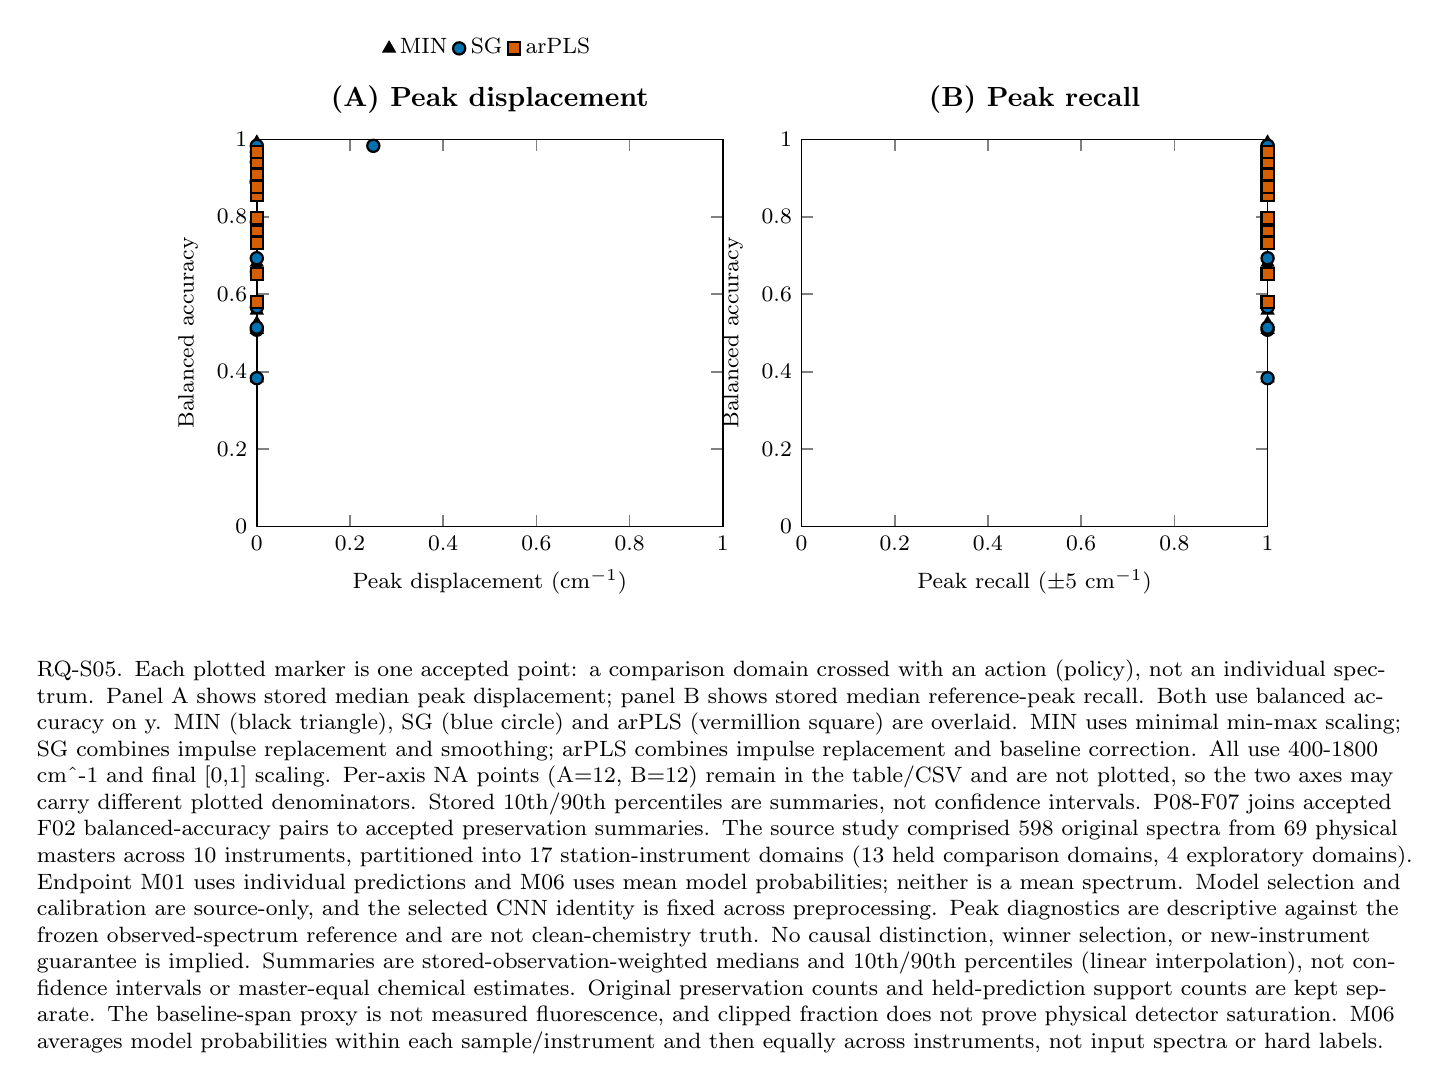
\begin{tikzpicture}
\begin{groupplot}[group style={group size=2 by 1, horizontal sep=10mm, vertical sep=0mm}, width=75mm, height=65mm, clip=false, axis line style={line width=0.6pt}, tick style={line width=0.6pt}, tick label style={font=\fontsize{8}{9.6}\selectfont, black}, label style={font=\fontsize{8}{9.6}\selectfont, black}, title style={font=\bfseries\fontsize{10}{12}\selectfont}, legend style={at={(0.5,1.18)}, anchor=south, draw=none, fill=none, legend columns=3, font=\fontsize{8}{9.6}\selectfont}, ymin=0, ymax=1, ytick={0,0.20000000000000001,0.40000000000000002,0.59999999999999998,0.80000000000000004,1}, yticklabels={0,0.2,0.4,0.6,0.8,1}]
\nextgroupplot[title={(A) Peak displacement}, xlabel={Peak displacement (cm$^{-1}$)}, ylabel={Balanced accuracy}, xmin=0, xmax=1, xtick={0,0.20000000000000001,0.40000000000000002,0.59999999999999998,0.80000000000000004,1}, xticklabels={0,0.2,0.4,0.6,0.8,1}]
\addlegendimage{only marks, mark=triangle*, mark size=2.2pt, mark options={fill=f07min, draw=black, line width=0.8pt}}
\addlegendentry{MIN}
\addlegendimage{only marks, mark=*, mark size=2.2pt, mark options={fill=f07sg, draw=black, line width=0.8pt}}
\addlegendentry{SG}
\addlegendimage{only marks, mark=square*, mark size=2.2pt, mark options={fill=f07arpls, draw=black, line width=0.8pt}}
\addlegendentry{arPLS}
\addplot+[only marks, mark=triangle*, mark size=2.2pt, mark options={fill=f07min, draw=black, line width=0.8pt}] coordinates {(0,0.52499999999999991) (0,0.55833333333333324) (0,0.65833333333333333) (0,0.89583333333333337) (0,0.96666666666666656) (0,0.38333333333333325) (0,0.96666666666666679) (0,0.99166666666666681) (0,0.5083333333333333) (0,0.68194444444444435) (0,0.93888888888888877) (0,0.87361111111111112) (0,0.7861111111111112)};
\addplot+[only marks, mark=*, mark size=2.2pt, mark options={fill=f07sg, draw=black, line width=0.8pt}] coordinates {(0,0.5083333333333333) (0,0.56666666666666654) (0,0.65833333333333333) (0,0.94166666666666676) (0,0.96666666666666656) (0,0.38333333333333325) (0,0.98333333333333339) (0.25,0.98333333333333339) (0,0.51388888888888884) (0,0.69305555555555542) (0,0.89166666666666661) (0,0.89027777777777783) (0,0.78611111111111098)};
\addplot+[only marks, mark=square*, mark size=2.2pt, mark options={fill=f07arpls, draw=black, line width=0.8pt}] coordinates {(0,0.76111111111111118) (0,0.65277777777777768) (0,0.7958333333333335) (0,0.93333333333333357) (0,0.95833333333333326) (0,0.90833333333333321) (0,0.94999999999999996) (0,0.94166666666666676) (0,0.5805555555555556) (0,0.73333333333333328) (0,0.96666666666666679) (0,0.85694444444444451) (0,0.87777777777777766)};
\nextgroupplot[title={(B) Peak recall}, xlabel={Peak recall ($\pm$5 cm$^{-1}$)}, ylabel={Balanced accuracy}, xmin=0, xmax=1, xtick={0,0.20000000000000001,0.40000000000000002,0.59999999999999998,0.80000000000000004,1}, xticklabels={0,0.2,0.4,0.6,0.8,1}]
\addplot+[only marks, mark=triangle*, mark size=2.2pt, mark options={fill=f07min, draw=black, line width=0.8pt}] coordinates {(1,0.52499999999999991) (1,0.55833333333333324) (1,0.65833333333333333) (1,0.89583333333333337) (1,0.96666666666666656) (1,0.38333333333333325) (1,0.96666666666666679) (1,0.99166666666666681) (1,0.5083333333333333) (1,0.68194444444444435) (1,0.93888888888888877) (1,0.87361111111111112) (1,0.7861111111111112)};
\addplot+[only marks, mark=*, mark size=2.2pt, mark options={fill=f07sg, draw=black, line width=0.8pt}] coordinates {(1,0.5083333333333333) (1,0.56666666666666654) (1,0.65833333333333333) (1,0.94166666666666676) (1,0.96666666666666656) (1,0.38333333333333325) (1,0.98333333333333339) (1,0.98333333333333339) (1,0.51388888888888884) (1,0.69305555555555542) (1,0.89166666666666661) (1,0.89027777777777783) (1,0.78611111111111098)};
\addplot+[only marks, mark=square*, mark size=2.2pt, mark options={fill=f07arpls, draw=black, line width=0.8pt}] coordinates {(1,0.76111111111111118) (1,0.65277777777777768) (1,0.7958333333333335) (1,0.93333333333333357) (1,0.95833333333333326) (1,0.90833333333333321) (1,0.94999999999999996) (1,0.94166666666666676) (1,0.5805555555555556) (1,0.73333333333333328) (1,0.96666666666666679) (1,0.85694444444444451) (1,0.87777777777777766)};
\end{groupplot}
\node[anchor=north, yshift=-6mm, text width=175mm, align=left, font=\fontsize{8}{9.6}\selectfont] at (current bounding box.south) {RQ-S05. Each plotted marker is one accepted point: a comparison domain crossed with an action (policy), not an individual spectrum. Panel A shows stored median peak displacement; panel B shows stored median reference-peak recall. Both use balanced accuracy on y. MIN (black triangle), SG (blue circle) and arPLS (vermillion square) are overlaid. MIN uses minimal min-max scaling; SG combines impulse replacement and smoothing; arPLS combines impulse replacement and baseline correction. All use 400-1800 cm\textasciicircum{}-1 and final [0,1] scaling. Per-axis NA points (A=12, B=12) remain in the table/CSV and are not plotted, so the two axes may carry different plotted denominators. Stored 10th/90th percentiles are summaries, not confidence intervals. P08-F07 joins accepted F02 balanced-accuracy pairs to accepted preservation summaries. The source study comprised 598 original spectra from 69 physical masters across 10 instruments, partitioned into 17 station-instrument domains (13 held comparison domains, 4 exploratory domains). Endpoint M01 uses individual predictions and M06 uses mean model probabilities; neither is a mean spectrum. Model selection and calibration are source-only, and the selected CNN identity is fixed across preprocessing. Peak diagnostics are descriptive against the frozen observed-spectrum reference and are not clean-chemistry truth. No causal distinction, winner selection, or new-instrument guarantee is implied. Summaries are stored-observation-weighted medians and 10th/90th percentiles (linear interpolation), not confidence intervals or master-equal chemical estimates. Original preservation counts and held-prediction support counts are kept separate. The baseline-span proxy is not measured fluorescence, and clipped fraction does not prove physical detector saturation. M06 averages model probabilities within each sample/instrument and then equally across instruments, not input spectra or hard labels.};
\end{tikzpicture}
\end{minipage}
\end{document}